\begin{figure}
\centering
\begin{subfigure}{0.45\textwidth}
    \centering
    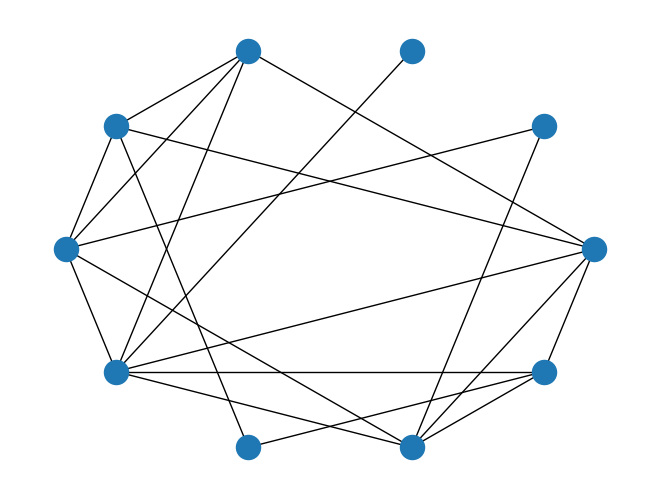
\includegraphics[width=\textwidth]{Figs/n=10_graph_1.png}
    \caption{Graph 1}
\end{subfigure}
\hfill
\begin{subfigure}{0.45\textwidth}
    \centering
    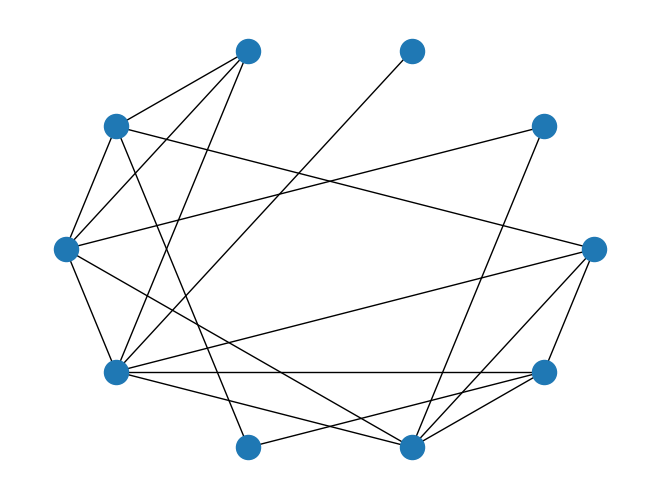
\includegraphics[width=\textwidth]{Figs/n=10_graph_2.png}
    \caption{Graph 2}
\end{subfigure}
\caption{The two graphs used in the first $n=10$ simulation.}
\label{fig:graphs}
\end{figure}

\begin{figure}
\centering
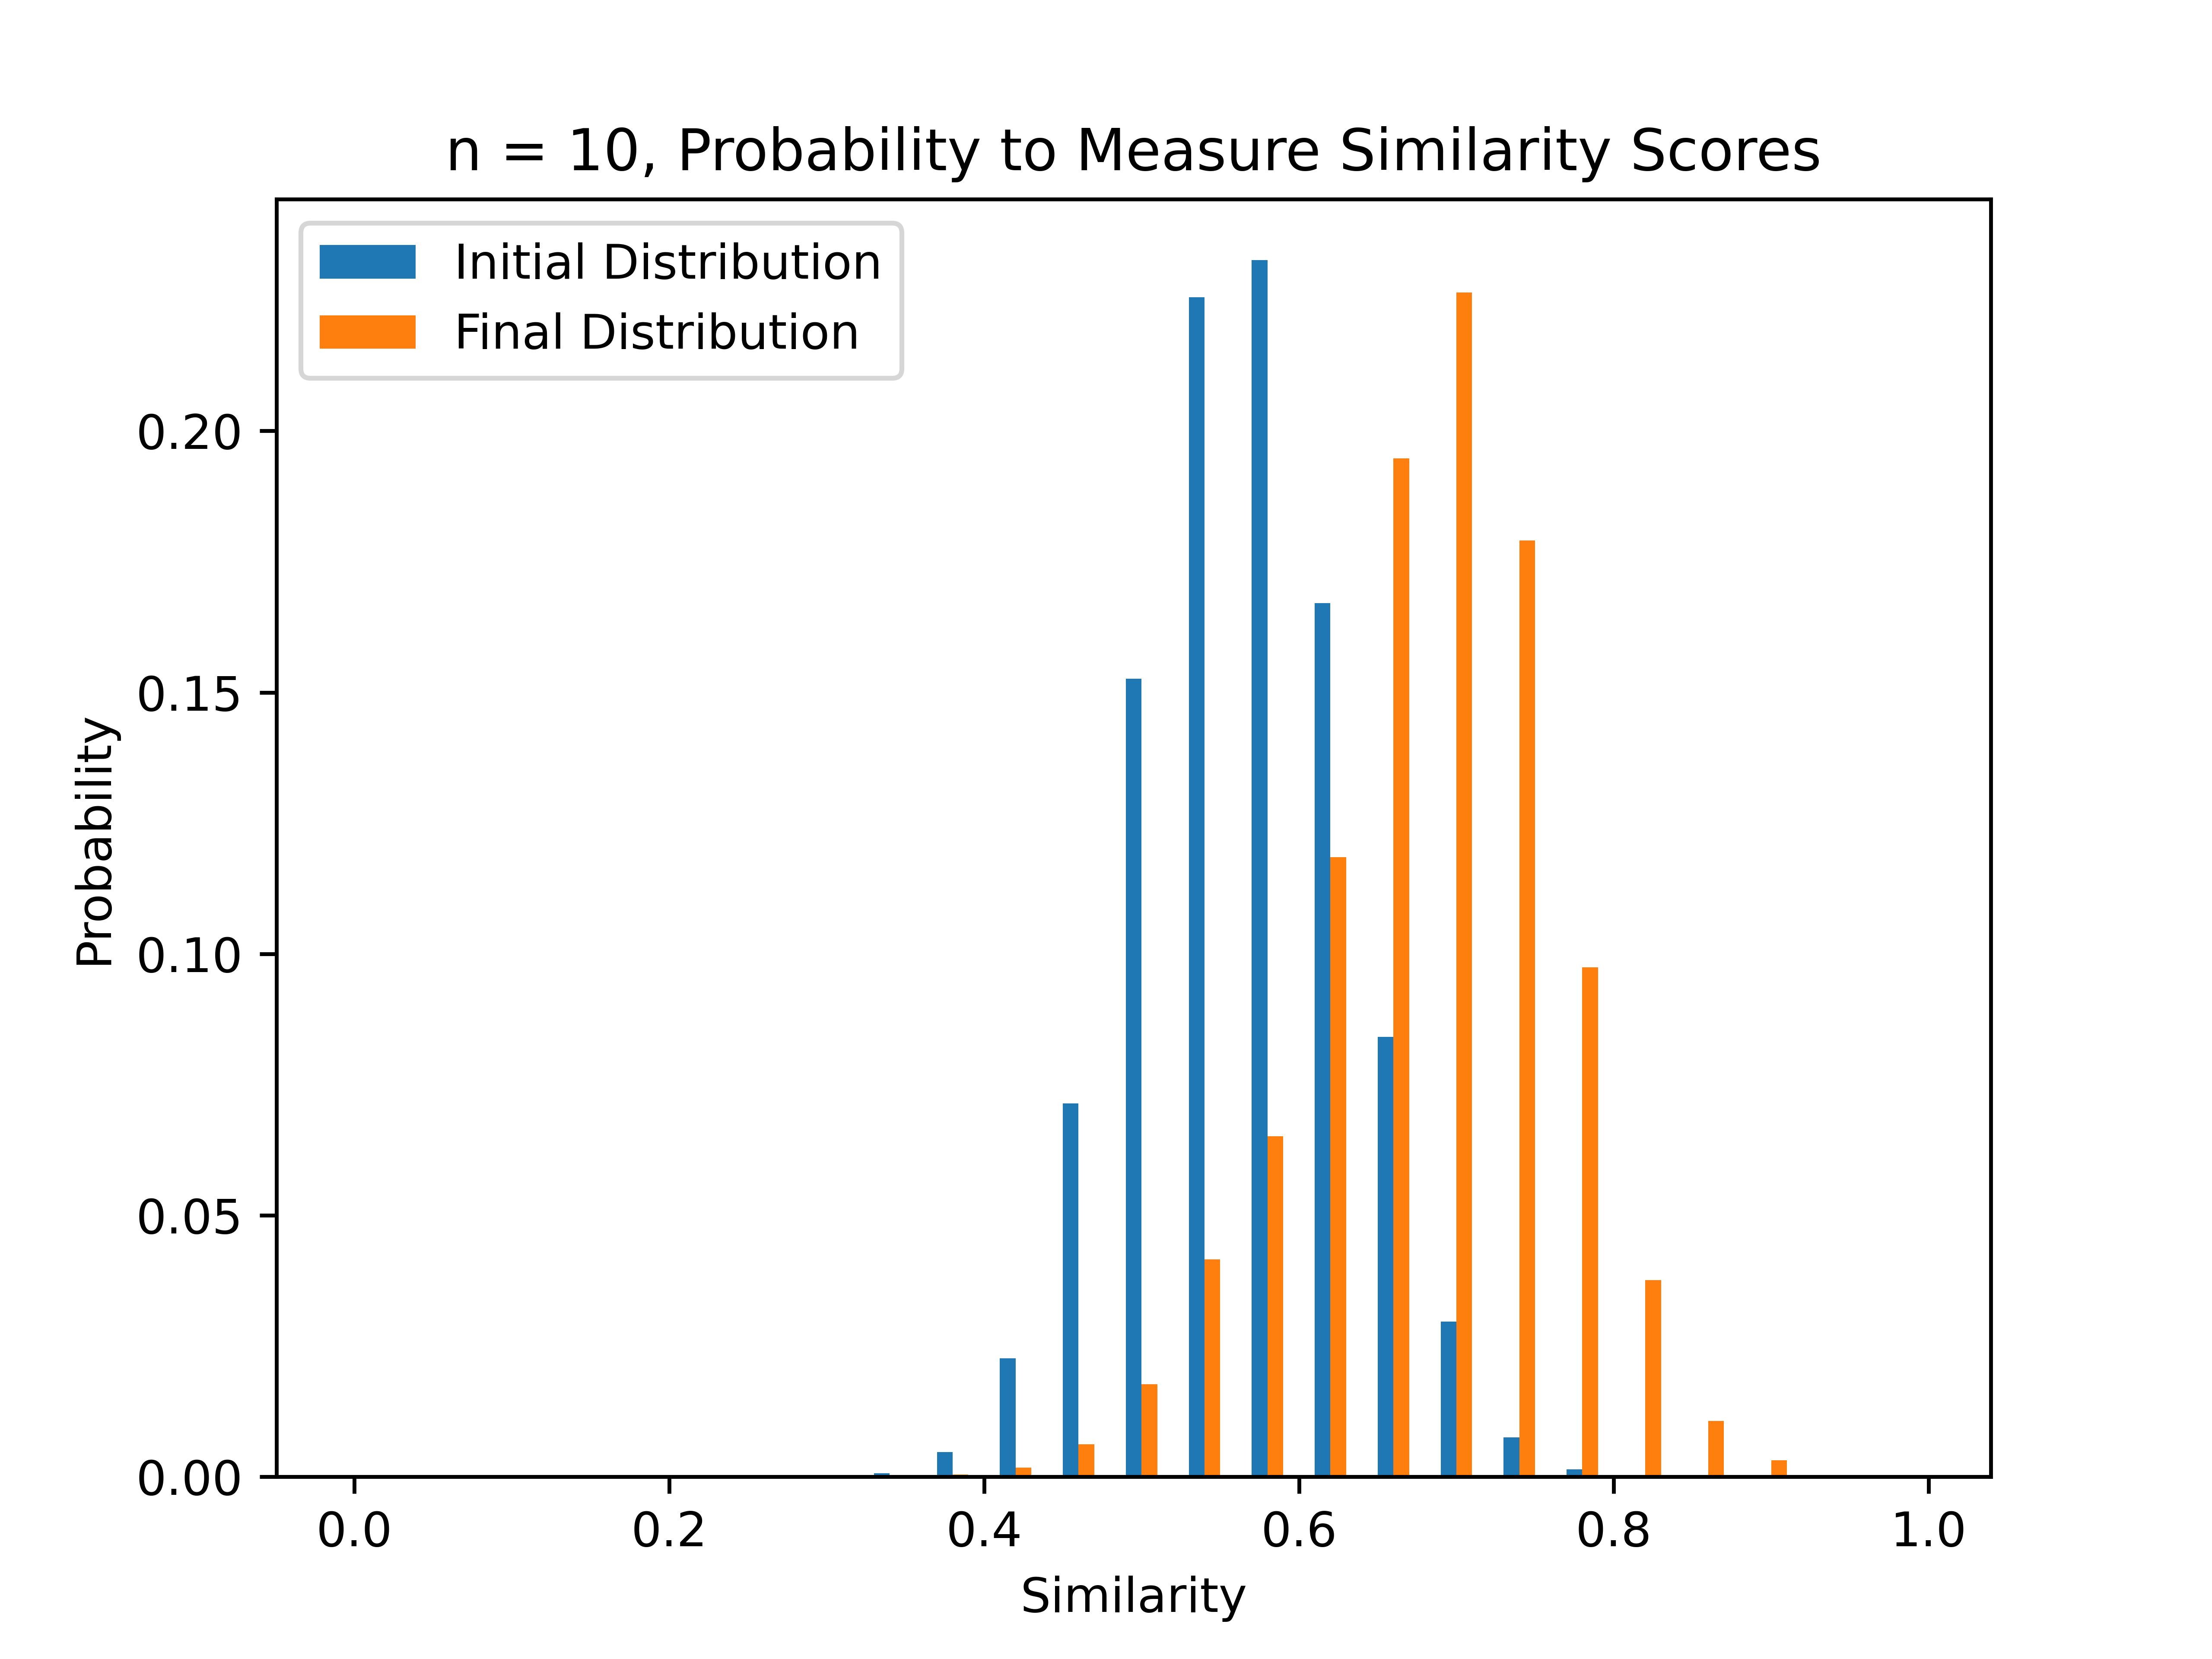
\includegraphics[width=0.75\textwidth]{Figs/n=10_Similarity_scores.png}
\caption{The initial and final probability distributions over similarity scores after 5 iterations for the $n=10$ case.}
\label{fig:similarity_scores}
\end{figure}

\begin{figure}
\centering
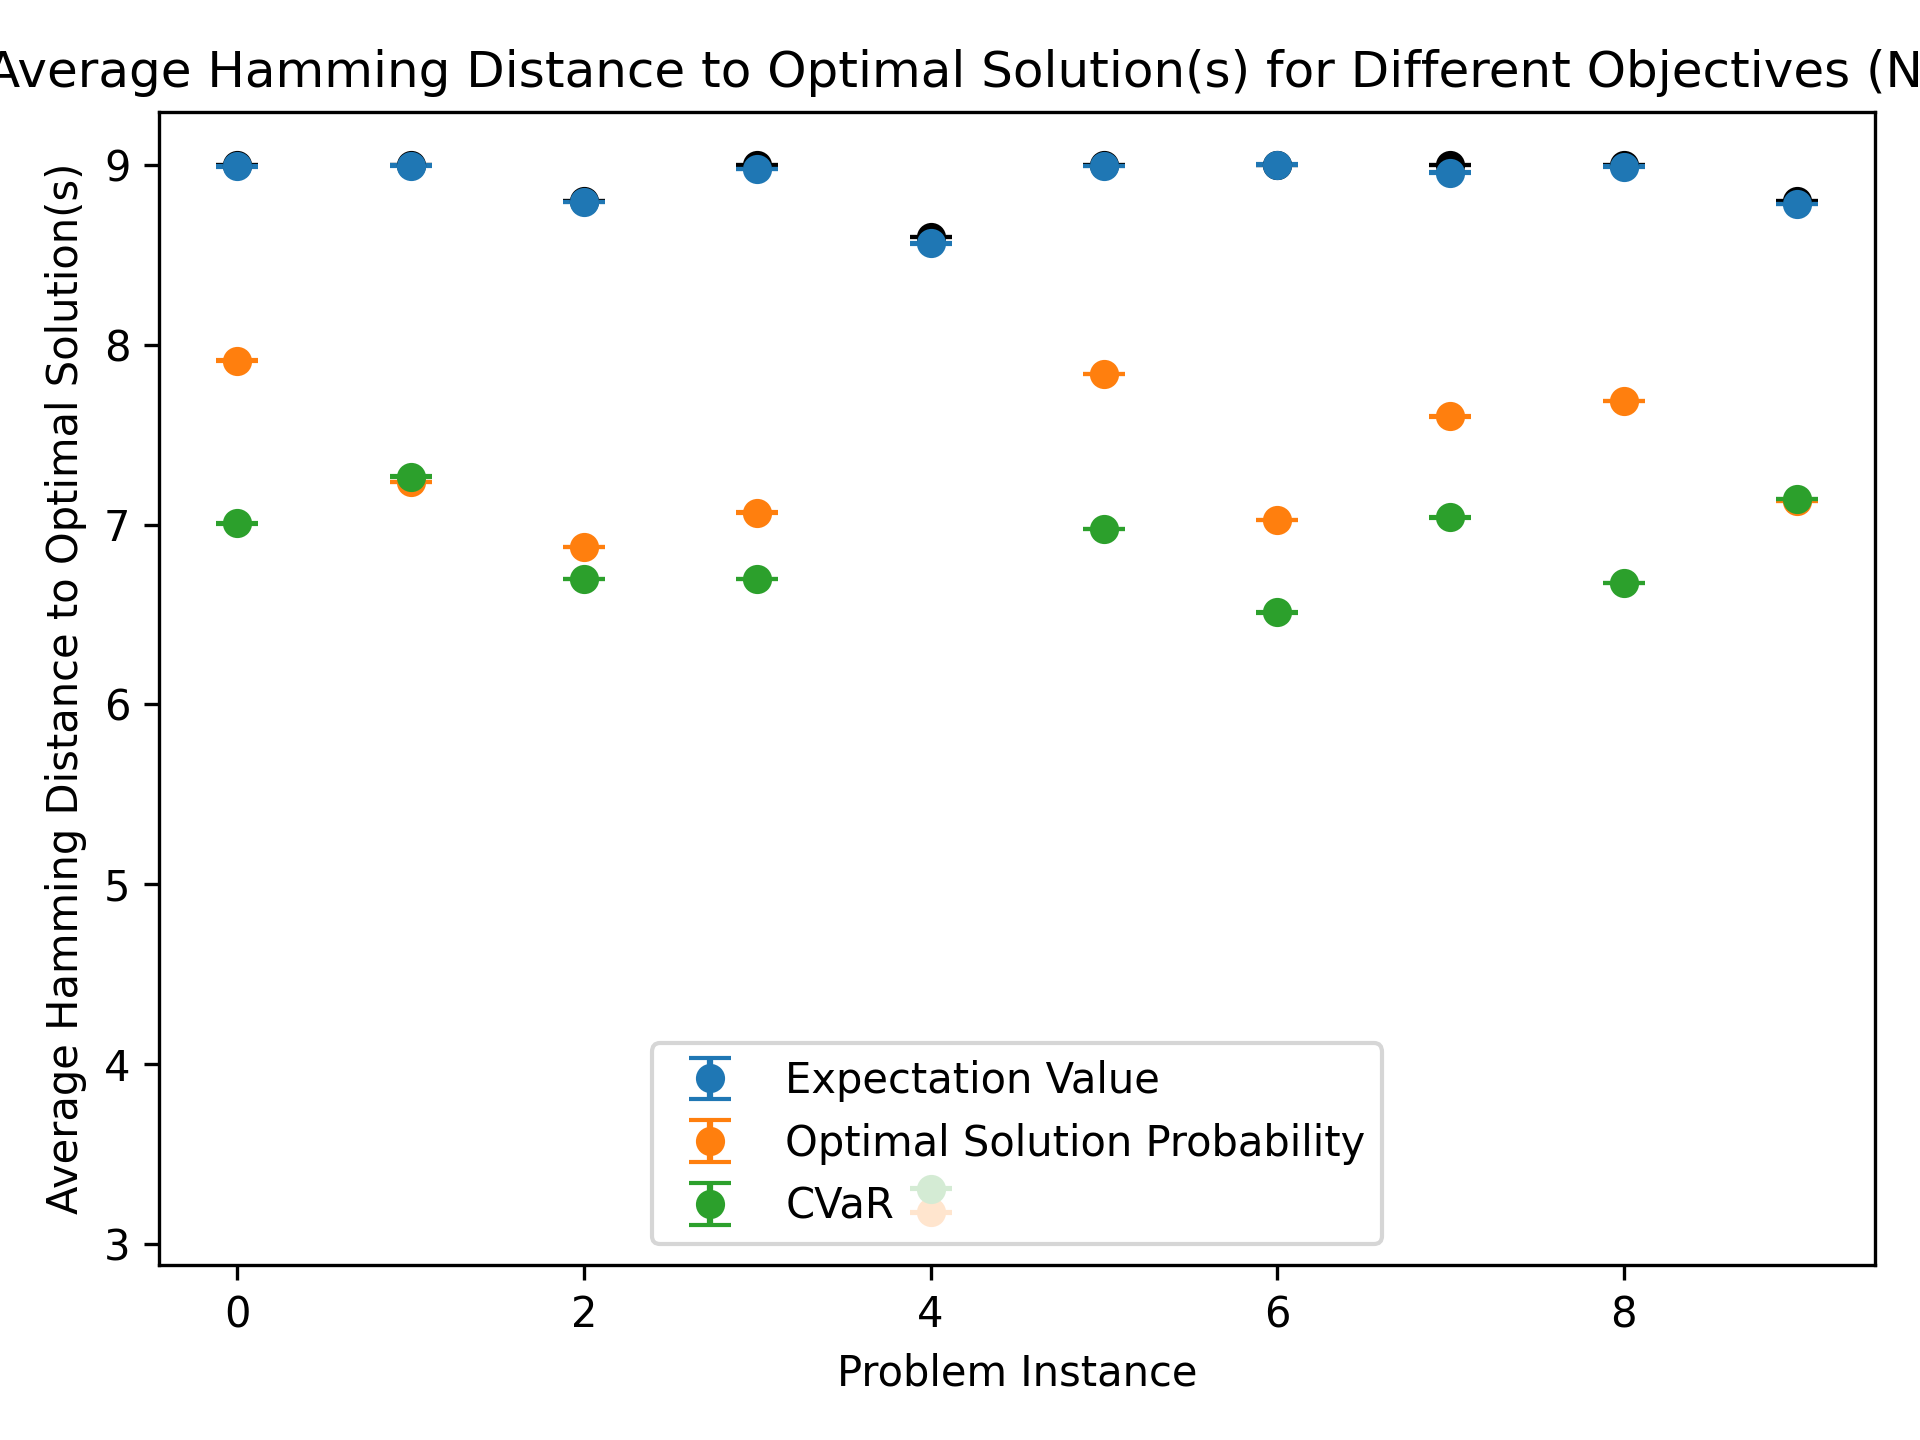
\includegraphics[width=0.75\textwidth]{Figs/avg_hamming_distance_comparison.png}
\caption{$n=10$}
\label{fig:all_hams}
\end{figure}

\begin{figure}
\centering
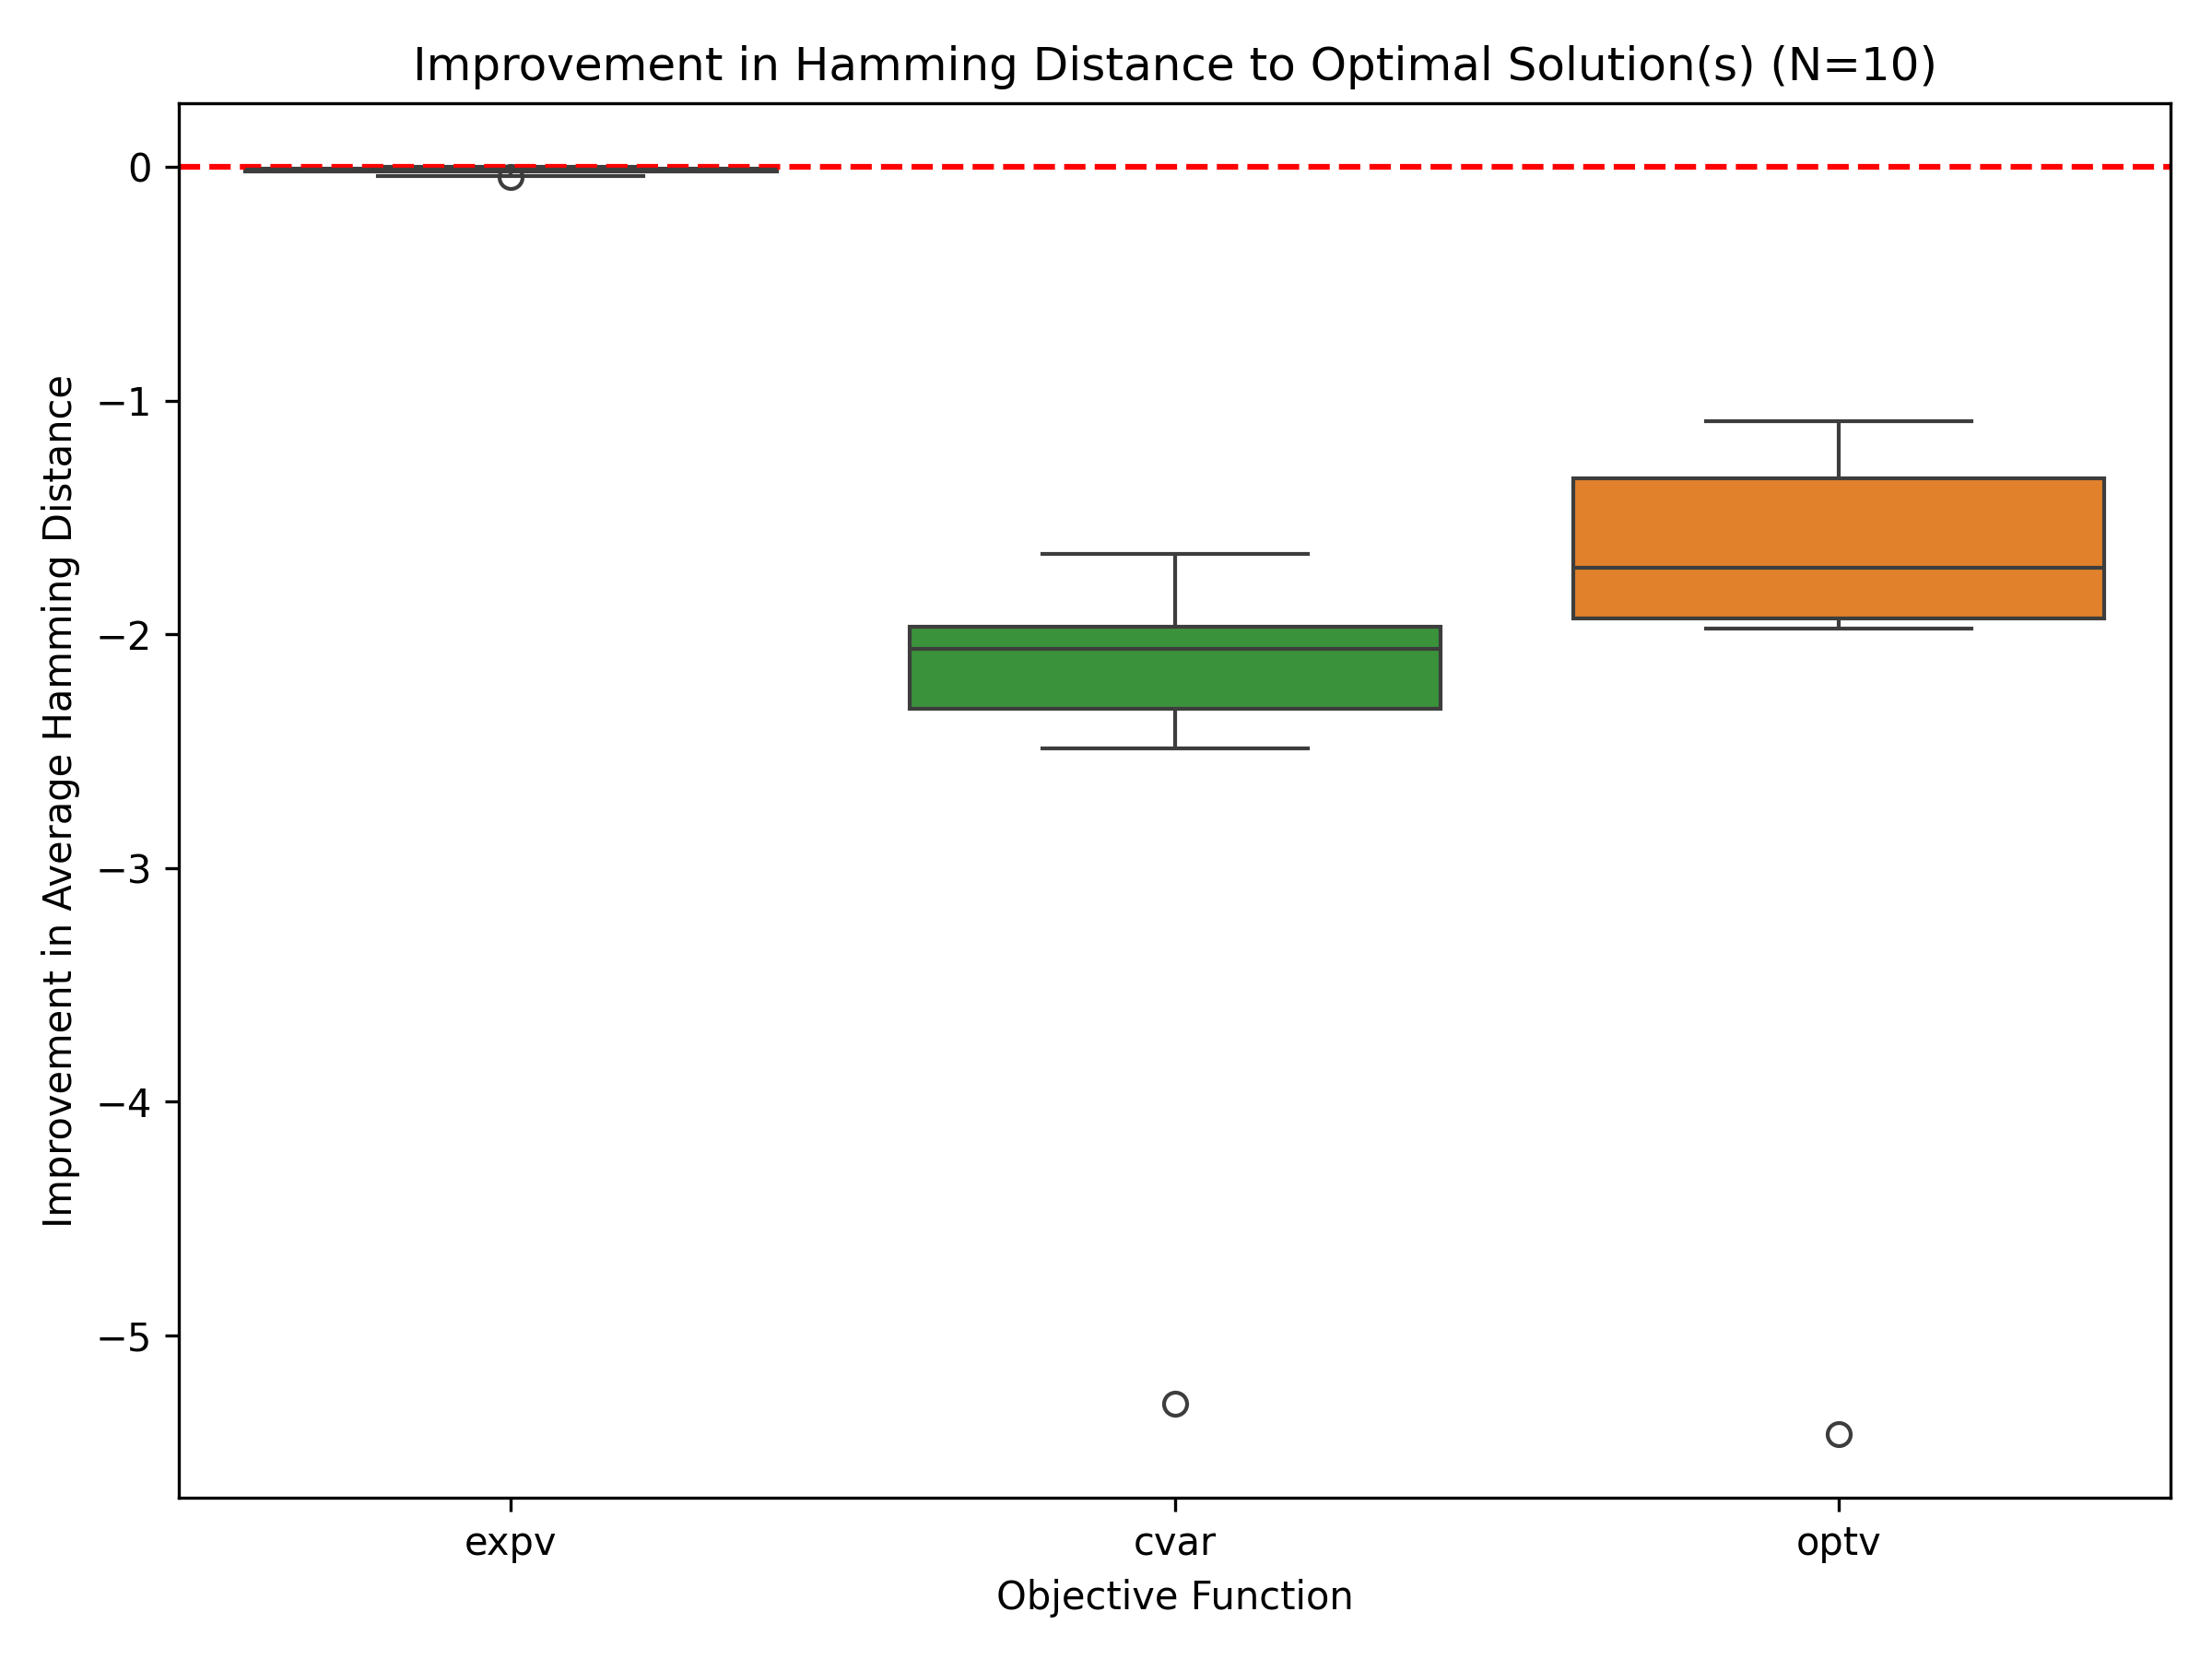
\includegraphics[width=0.75\textwidth]{Figs/hamming_distance_improvement_boxplot.png}
\caption{Improvement in mean hamming distancec $n=10$}
\label{fig:ham_improvement}
\end{figure}

\begin{figure}
\centering
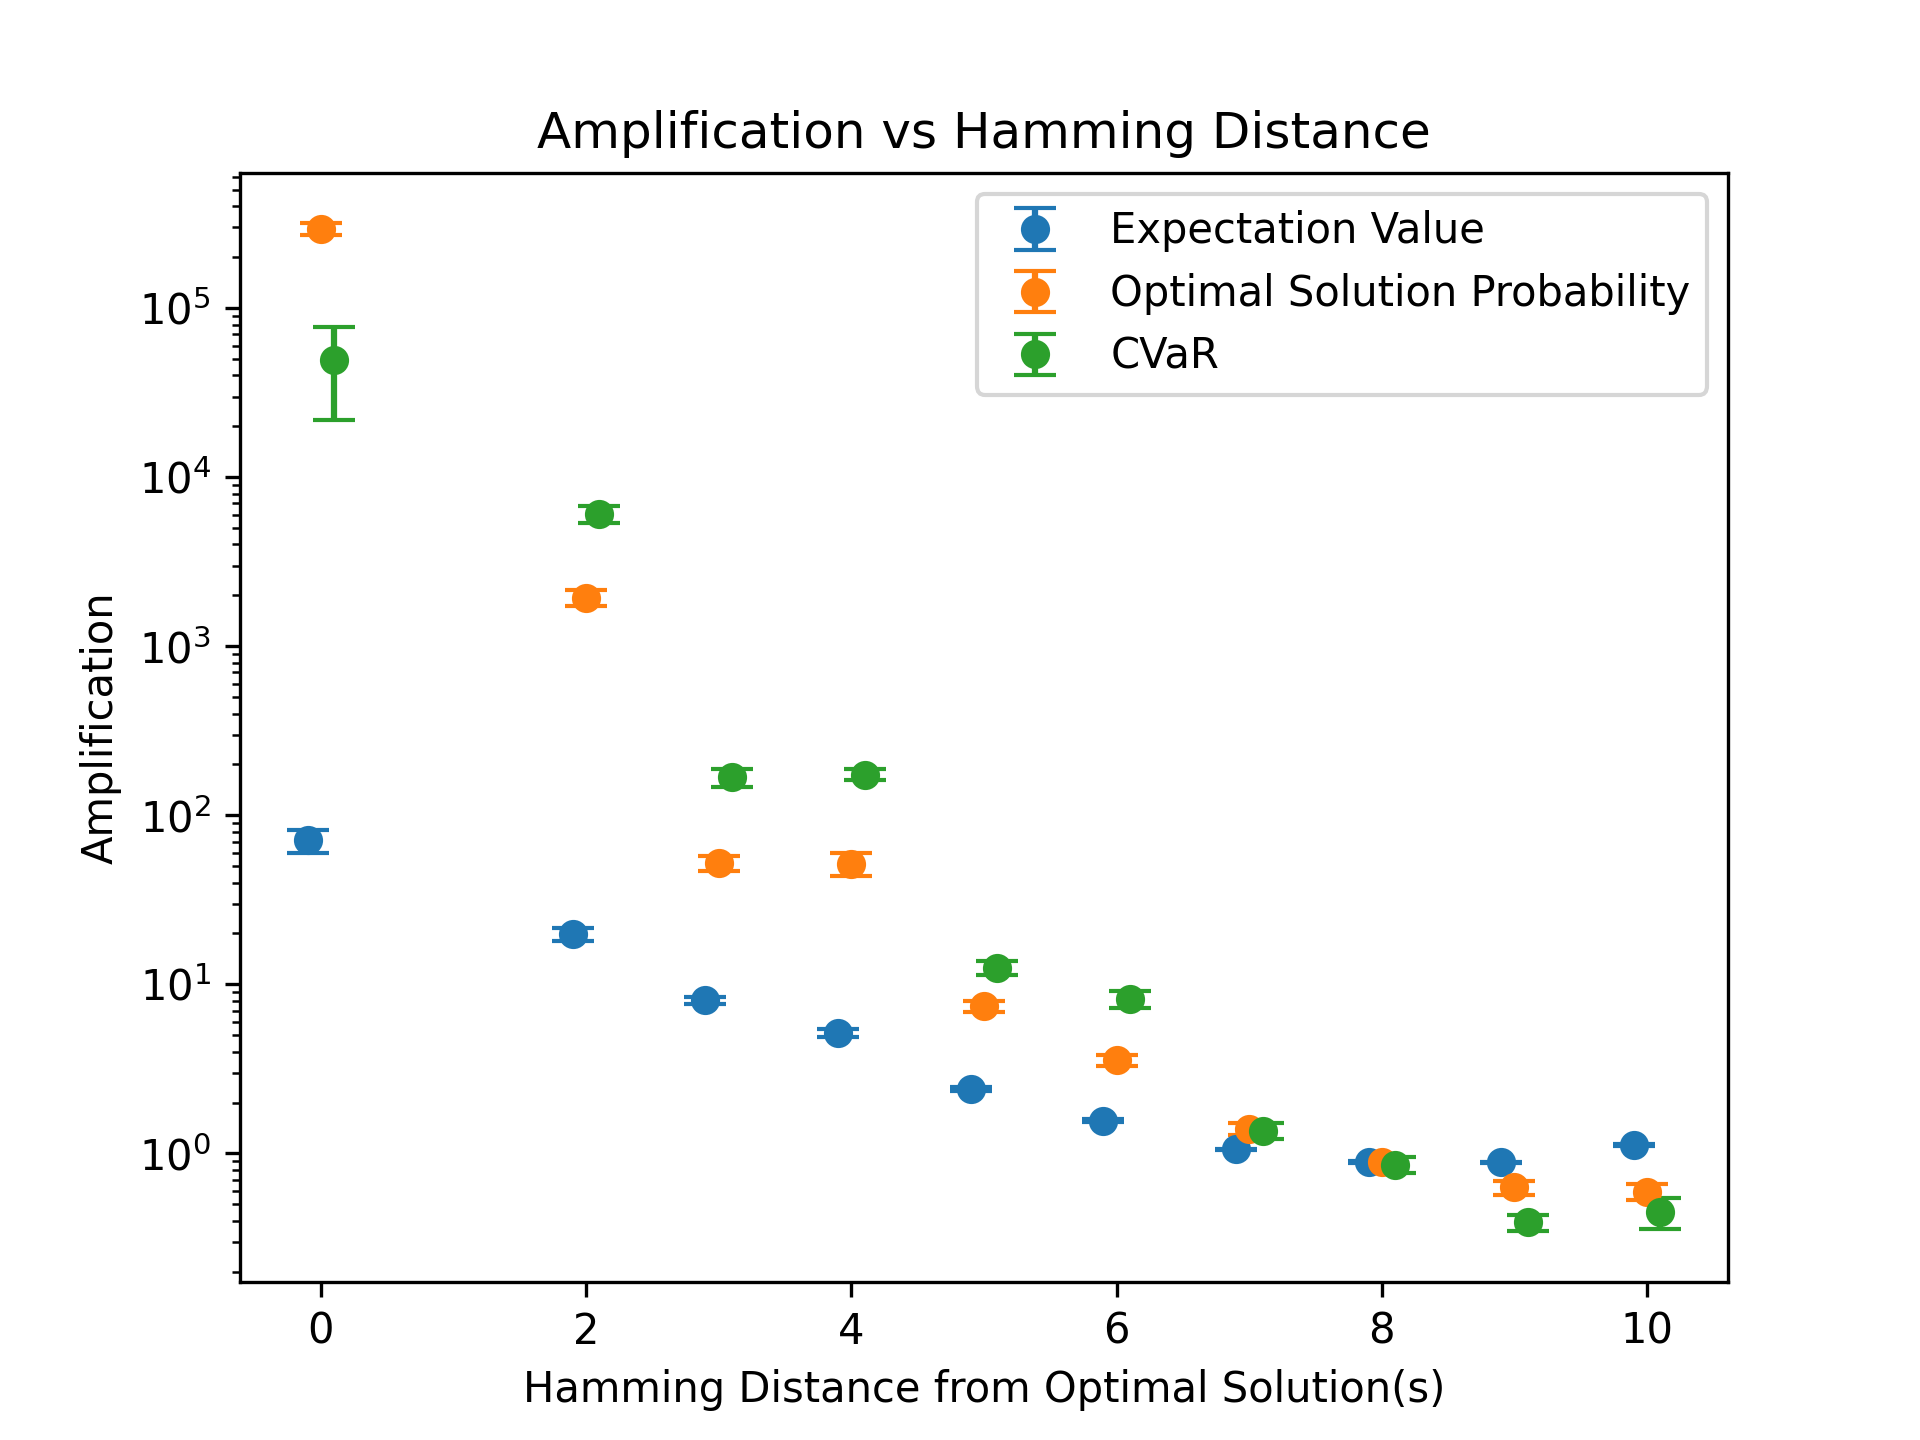
\includegraphics[width=0.75\textwidth]{Figs/amplification_vs_hamming_distance.png}
\caption{$n=10$}
\label{fig:ham_amplification}
\end{figure}